\usepackage{ifthen}
\usepackage{xstring}

\newcommand{\shrinktofit}[2]{\resizebox{#1}{!}{#2}}

\newcommand{\createBackground}[2]{
	\backgroundsetup{
		scale=1,
		color=black,
		opacity=1,
		angle=0,
		contents={
				\begin{tikzpicture}[remember picture,overlay]
					% Wood background
					\node[anchor=south west,inner sep=0] (background) at (current page.south west) {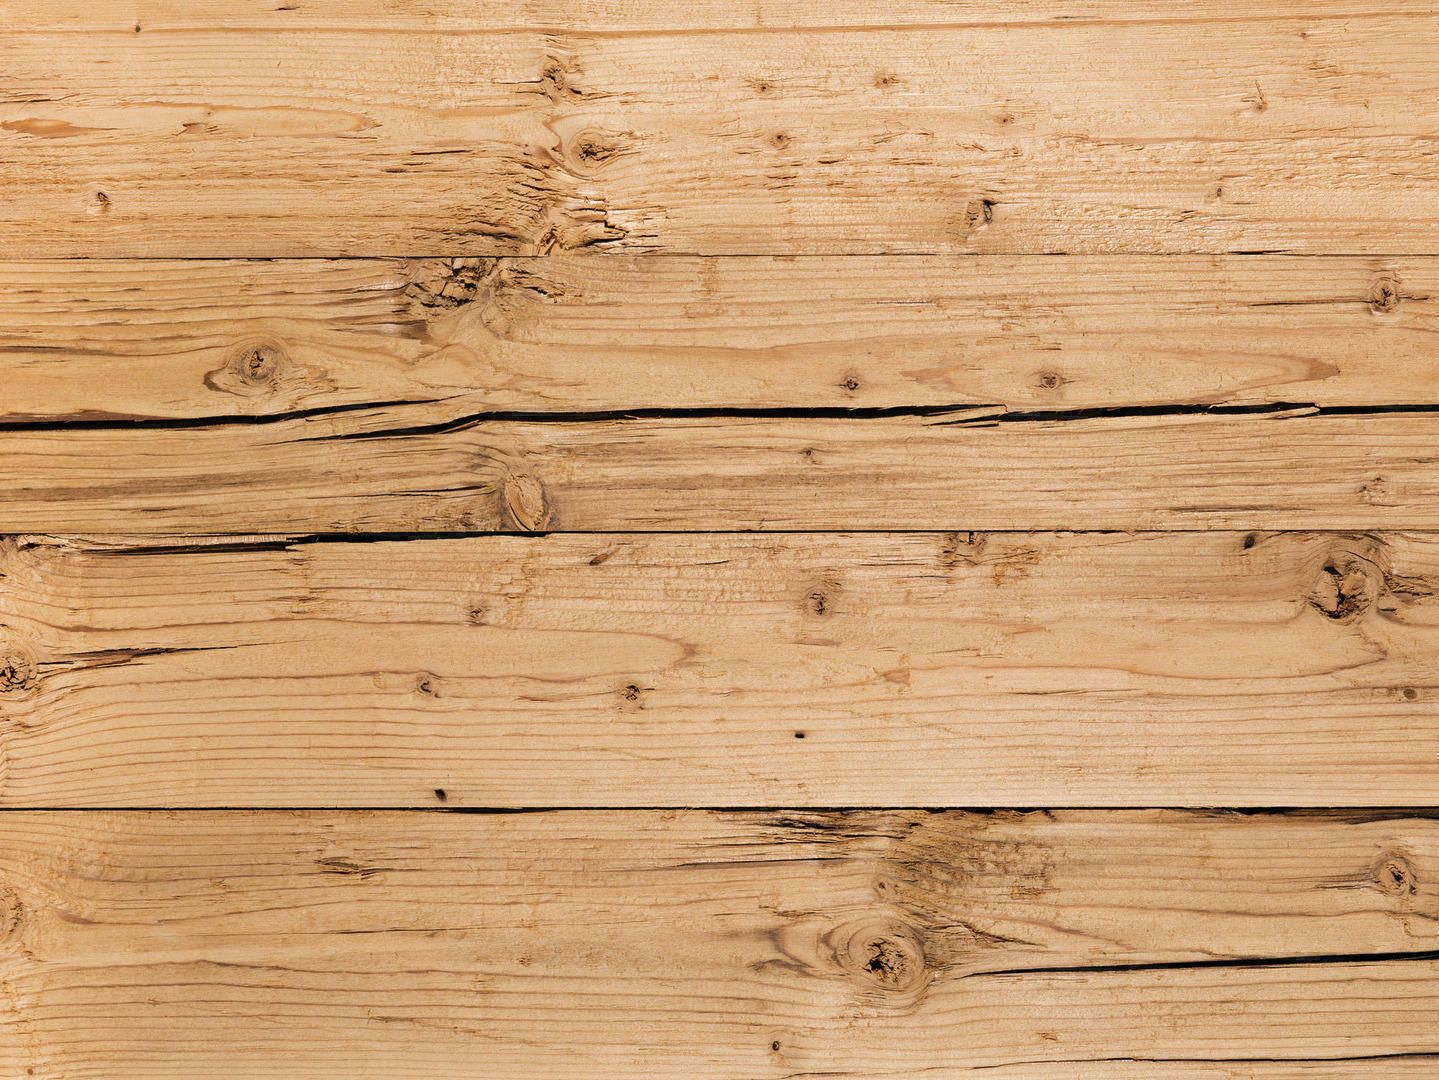
\includegraphics[width=\paperwidth,height=\paperheight]{./images/wood.JPG}};
					% Outer book cover
					\fill[bookcolor, drop shadow={shadow xshift=0.05cm, shadow yshift=-0.05cm, fill=black, opacity=0.5}] ([xshift=0.6cm,yshift=0.6cm]current page.south west) rectangle ([xshift=-0.6cm,yshift=-0.6cm]current page.north east);
					% Left black rectangle (paper page) with adjusted opacity and offset
					\fill[black, opacity=0.5] ([xshift=1.25cm,yshift=1.15cm]current page.south west) rectangle ([xshift=-0.5\paperwidth-0.05cm,yshift=-1.25cm]current page.north east);
					% Right black rectangle (paper page) with adjusted opacity and offset
					\fill[black, opacity=0.5] ([xshift=0.5\paperwidth+0.2cm,yshift=1.15cm]current page.south west) rectangle ([xshift=-1.15cm,yshift=-1.25cm]current page.north east);
					% Marker for navigation
					\foreach \name [count=\i] in \Girls {
						\draw[rounded corners, fill=black, opacity=0.5] ([xshift=.3cm,yshift=-.55cm-\i*0.825cm]current page.north west) ([xshift=1.55cm,yshift=-1.3cm-\i*0.825cm]current page.north west);
						\draw[rounded corners, fill=markerGirls, draw=black] ([xshift=.25cm,yshift=-.5cm-\i*0.825cm]current page.north west) rectangle ([xshift=1.5cm,yshift=-1.25cm-\i*0.825cm]current page.north west);
						\StrLen{\name}[\textlength]
						% Check if the text is longer than 0 characters
						\ifthenelse{\textlength > 0}{%
							% The text is longer than 0 characters and contains \mytextlength\ characters.%
							\node[anchor=west] at ([xshift=.28cm,yshift=-0.825cm-\i*0.825cm]current page.north west) {\tiny\ComingSoon\textcolor{white}\name};
						}{}
						\node[draw, fill=white, opacity=0, anchor=north west] at ([xshift=.25cm,yshift=-.5cm-\i*0.825cm]current page.north west) [minimum width=1cm, minimum height=0.75cm] {
							\hyperlink{Girls\i}{\tikz\node[draw, fill=red, opacity=0, minimum width=1cm, minimum height=0.75cm]  {};}
						};
					}
					\foreach \name [count=\i] in \Boys {
						\draw[rounded corners, fill=black, opacity=0.5] ([xshift=-.2cm,yshift=-.55cm-\i*0.825cm]current page.north east) rectangle ([xshift=-1.45cm,yshift=-1.3cm-\i*0.825cm]current page.north east);
						\draw[rounded corners, fill=markerBoys, draw=black] ([xshift=-.25cm,yshift=-.5cm-\i*0.825cm]current page.north east) rectangle ([xshift=-1.5cm,yshift=-1.25cm-\i*0.825cm]current page.north east);
						\StrLen{\name}[\textlength]
						% Check if the text is longer than 0 characters
						\ifthenelse{\textlength > 0}{%
							% The text is longer than 0 characters and contains \mytextlength\ characters.%
							\node[anchor=west] at ([xshift=-1.18cm,yshift=-0.825cm-\i*0.825cm]current page.north east) {\tiny\ComingSoon\textcolor{white}\name};
						}{}
						\node[draw=none, fill=none, anchor=north east] at ([xshift=-0.25cm, yshift=-0.5cm-\i*0.825cm]current page.north east) {
							\hyperlink{Boys\i}{\tikz\node[draw=none, fill=none, minimum width=1cm, minimum height=0.75cm] {};}
						};
					}
					% Left white rectangle (paper page)
					\fill[white] ([xshift=1.2cm,yshift=1.2cm]current page.south west) rectangle ([xshift=-0.5\paperwidth-0.1cm,yshift=-1.2cm]current page.north east);
					% Right white rectangle (paper page)
					\fill[white] ([xshift=0.5\paperwidth+0.15cm,yshift=1.2cm]current page.south west) rectangle ([xshift=-1.2cm,yshift=-1.2cm]current page.north east);
					% Add points to the left white rectangle
					\begin{scope}
						\clip ([xshift=1.2cm,yshift=1.2cm]current page.south west) rectangle ([xshift=-0.5\paperwidth-0.2cm,yshift=-1.2cm]current page.north east);
						\node at ([xshift=-0.25\paperwidth]current page.center) {\usebox\PaperPaternbox};
					\end{scope}
					% Add points to the right white rectangle
					\begin{scope}
						\clip ([xshift=0.5\paperwidth+0.15cm,yshift=1.2cm]current page.south west) rectangle ([xshift=-1.2cm,yshift=-1.2cm]current page.north east);
						\node at ([xshift=0.25\paperwidth]current page.center) {\usebox\PaperPaternbox};
					\end{scope}
					% Inner book cover
					\node[anchor=center,inner sep=0] at (current page.center) {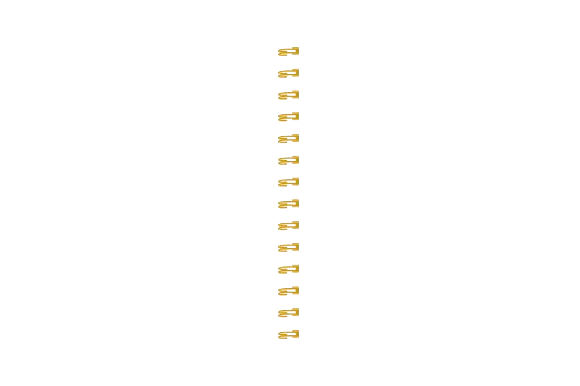
\includegraphics[width=\paperwidth,height=\paperheight]{./images/ringbinder.png}};
					% Make the current page bookmark bigger
					\ifthenelse{\NOT\equal{#1}{}}{
						\draw[rounded corners, fill=black, opacity=0.5] ([xshift=.3cm,yshift=-.55cm-#1*0.825cm]current page.north west) rectangle ([xshift=1.55cm,yshift=-1.3cm-#1*0.825cm]current page.north west);
						\draw[rounded corners, fill=markerGirls, draw=black] ([xshift=.25cm,yshift=-.5cm-#1*0.825cm]current page.north west) rectangle ([xshift=1.5cm,yshift=-1.25cm-#1*0.825cm]current page.north west);
						% \node[anchor=west] at ([xshift=.25cm,yshift=-0.825cm-\i*0.825cm]current page.north west) {\hyperlink{Girls\i}{\tiny\ComingSoon\textcolor{white}\name}};
						\StrLen{\name}[\textlength]
						% Check if the text is longer than 0 characters
						\ifthenelse{\textlength > 0}{%
							\node[anchor=west] at ([xshift=.28cm,yshift=-0.825cm-#1*0.825cm]current page.north west) {\tiny\ComingSoon\textcolor{white}\name};
						}{ }
					}{
						% Check if the second parameter is not empty
						\ifthenelse{\NOT\equal{#2}{}}{
							\draw[rounded corners, fill=black, opacity=0.5] ([xshift=-.2cm,yshift=-.55cm-#2*0.825cm]current page.north east) rectangle ([xshift=-1.45cm,yshift=-1.3cm-#2*0.825cm]current page.north east);
							\draw[rounded corners, fill=markerBoys, draw=black] ([xshift=-.25cm,yshift=-.5cm-#2*0.825cm]current page.north east) rectangle ([xshift=-1.5cm,yshift=-1.25cm-#2*0.825cm]current page.north east);
							\StrLen{\name}[\textlength]
							% Check if the text is longer than 0 characters
							\ifthenelse{\textlength > 0}{%
								\node[anchor=west] at ([xshift=-1.43cm,yshift=-0.825cm-#2*0.825cm]current page.north east) {\tiny\ComingSoon\textcolor{white}\name};
							}{ }
						}{}
					}
				\end{tikzpicture}
			}
	}
}
